\chapter{PENGUJIAN DAN ANALISIS}
\label{chap:pengujiananalisis}

% Ubah bagian-bagian berikut dengan isi dari pengujian dan analisis

Penelitian dilakukan dengan melakukan uji dan anaisa dari sistem yang telah dibuat berdasarkan langkah pada metodologi yang telah dilaksanakan. Pengujian ini dilakukan untuk menguji kemampuan sistem yang telah dibuat dalam menjawab permasalahan yang dijadikan acuan pada penelitian ini untuk mendapatkan hasil dari tujuan yang ingin didapat. Pembahasan pengujian yang dilakukan pada penelitian ini meliputi pengujian hasil \emph{training} dan \emph{validation} model, pengujian hasil \emph{testing} model, dan pengujian prediksi.

\section{Pengujian Hasil \emph{Ttraining} dan \emph{Validation} Model}
\label{sec:PengujianTrainingValidation}

Pengujian pembuatan model berdasarkan hasil \emph{training} dan \emph{validation} dengan menggunakan dataset dengan jumlah keseluruhan yaitu 1731 sampel data. Dengan jumlah sample training sebanyak 1385 dan sampel validation sebanyak 346. Setelah dilakukan proses \emph{training} dan \emph{validation} terhadap dataset yang telah ditentukan oleh sampel data, didapatkan hasil pengujian akurasi dengan tingkat akurasi training sebesar 96\% dan tingkat akurasi validation sebesar 96\%. Kemudian didapatkan hasil pengujian loss pada training sebesar 0,4\% dan loss pada validation sebesar 0,4\%. Hasil pengujian ditunjukkan pada grafik nilai akurasi dan loss pada proses \emph{training} dan \emph{validation} seperti pada Gambar \ref{fig:HasilTrainingValidation}.

\begin{figure}[H]
  \centering
  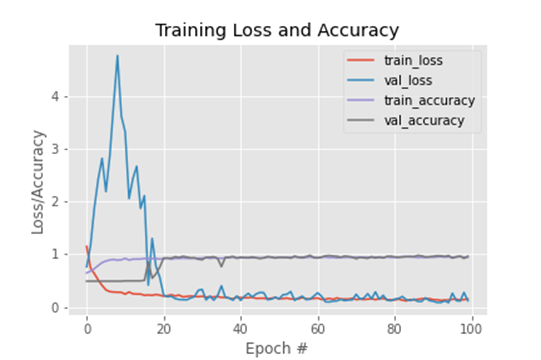
\includegraphics[scale=0.85]{gambar/hasil training dan validation.png}
  \caption{Grafik hasil \emph{training} dan \emph{validation}}
  \label{fig:HasilTrainingValidation}
\end{figure}


\section{Pengujian Testing Model}
\label{sec:PengujianTestingModel}

Pengujian dilanjutkan dengan melakukan \emph{testing} model dengan menggunakan dataset yang sudah dimiliki dengan jumlah keseluruhan yaitu 1731 sampel data. Hasil pengujian \emph{testing} model didapatkan akurasi sebesar 45\% dengan hasil deteksi benar untuk kelas kanan sebanyak 410 sampel (46\%) dan kelas kiri sebanyak 380 sampel (44\%). Pengujian ditunjukkan dengan confusion matrix pada Gambar \ref{fig:HasilTesting} dan Tabel \ref{tb:ClassificationReport} merupakan classification report dari hasil pengujian yang telah dilakukan pada pengujian \emph{testing} model penelitian ini.

\begin{figure}[H]
  \centering
  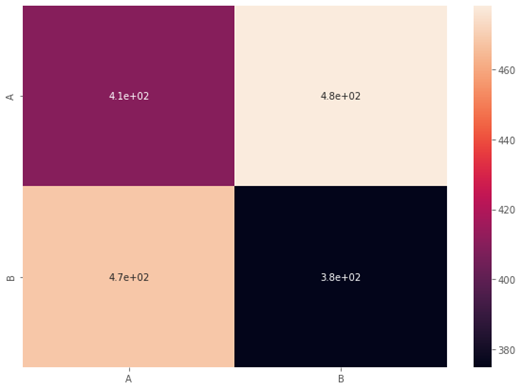
\includegraphics[scale=0.8]{gambar/hasil confusion matrix.png}
  \caption{\emph{Confusion Matrix} hasil \emph{testing} model}
  \label{fig:HasilTesting}
\end{figure}

\begin{longtable}{|c|c|c|c|c|}
  \caption{\emph{Classification Report} hasil pengujian \emph{testing} model}
  \label{tb:ClassificationReport}                                   \\
  \hline
  \rowcolor[HTML]{C0C0C0}
   & \textbf{Precision} & \textbf{Recall} & \textbf{F1-Score} & \textbf{Support} \\
  \hline
  kanan     & 0,47    & 0,46    & 0,46    & 888         \\
  \hline
  kiri      & 0,44    & 0,44    & 0,46    & 843           \\
  \hline
  Accuracy  &         &         & 0,45    & 1731            \\
  \hline
\end{longtable}


\section{Pengujian Prediksi}
\label{sec:PengujianPrediksi}

Pengujian pada prediksi jumlah kalori yang terbakar dilakukan setelah melakukan pengujian pada model deteksi yang telah dilakukan. Prediksi dilakukan dengan dua metode, yaitu regresi linear dan perhitungan rumus. Dengan menggunakan dataset berupa citra video yang akan digunakan untuk melakukan prediksi kalori sebanyak 6 sampel video sehingga terdapat 6 percobaan yang dilakukan. Hasil yang diperoleh melalui model yang telah dibuat untuk deteksi dan melakukan prediksi sesuai metode yang dilakukan didapatkan hasil akumulasi kalori dengan prediksi regresi sebesar 93,61\% dengan akumulasi error sebesar 6,39\%. Kemudian prediksi dengan perhitungan rumus didapatkan hasil akumulasi kalori sebesar 00,00\% dengan akumulasi error sebesar 0,00\%. Tabel \ref{tb:PengujianPrediksi} merupakan hasil perbandingan antara dataset percobaan dengan nilai kalori pembanding dataset dengan proses prediksi.

\begin{longtable}{|c|c|c|c|c|}
  \caption{Pengujian Hasil Prediksi Kalori}
  \label{tb:PengujianPrediksi}                                   \\
  \hline
  \rowcolor[HTML]{C0C0C0}
  \textbf{Percobaan} & \textbf{Kecepatan} & \textbf{Kalori Treadmill} & \textbf{Prediksi Regresi} & \textbf{Perhitungan MET} \\
  \hline
  1   & 3     & 10    & 11,652    & 6,788   \\
  \hline
  2   & 6     & 10    & 8,245     & 4,744   \\
  \hline
  3   & 9     & 20    & 20,534    & 22,462   \\
  \hline
  4   & 12    & 20    & 19,927    & 20,575   \\
  \hline
  5   & 8     & 20    & 20,14     & 22,126   \\
  \hline
  6   & 12    & 20    & 20,056    & 19,331   \\
  \hline
\end{longtable}